\renewcommand{\newCommandChapterTitle}{Implementación de OCS-WAF}
\chapter{\newCommandChapterTitle}
\markright{\hfill \thechapter. \newCommandChapterTitle}
\label{chap:p3_new_waf}


Este capítulo presenta los detalles de implementación de \gls{acr3:name},
un \gls{acr3:waf} que utiliza los componentes descritos en los capítulos
anteriores para la detección de mensajes \gls{acr3:http} anómalos.
Iniciaremos este capítulo explicando algunos conceptos sobre \gls{acr3:waf}s
y detección de anomalías, luego presentamos la arquitectura general de
nuestra implementación y después describimos el funcionamiento de la misma
durante las fases de entrenamiento y detección, detallando los pasos
intermedios presentes en cada una de las dos fases.

El código fuente de nuestra implementación está disponible en nuestro
repositorio público bajo la dirección \TheRepoUrl.


\section{Detección de intrusiones con \textit{Web Application Firewalls}}

Los sistemas de detección de intrusión (\gls{acr3:ids} -
\textit{Intrusion Detection System}) son programas o dispositivos
especializados para monitorear las actividades en un sistema en busca
de intrusiones no autorizadas o posibles ataques, siendo un elemento
fundamental y necesario para garantizar la seguridad del sistema
\citep{scarfone2007guide}. % from section 2 - IDS and IPS principles

Se pueden utilizar tres criterios principales para clasificar los
\gls{acr3:ids}, en primer lugar según los modos de respuesta que utilizan
frente a intrusiones, en segundo lugar según las fuentes de datos que
emplean para sus análisis y en tercer lugar se los puede clasificar según
la metodología de detección que usan
\citep{torranoGimenez2015study}. % from section 2.2.1 - IDS classification
A continuación damos una breve explicación de los \gls{acr3:ids} según
cada uno de estos criterios de clasificación, resaltando las características
más relevantes de cada caso.

\begin{itemize}
    \item
    De acuerdo al modo de respuesta del sistema, se puede tener:

    \begin{itemize}
        \item
        \textit{Intrusion Detection System} (\gls{acr3:ids}):
        esta clase de sistema actúa de forma pasiva y solamente lanza
        alertas o mensajes cuando detecta actividades no autorizadas,
        pero no realiza acciones de contención.

        \item
        \textit{Intrusion Prevention System} (\gls{acr3:ips}):
        este tipo de sistema trabaja de forma activa para prevenir
        intrusiones y está equipado con herramientas para mitigar los
        daños de posibles ataques.
    \end{itemize}

    \item
    De acuerdo a las fuentes de datos para el análisis, se puede tener:

    \begin{itemize}
        \item
        \textit{Host-based systems} (\gls{acr3:hids}):
        esta clase de sistema analiza las actividades de máquinas
        individuales, monitoreando diferentes aspectos de las mismas,
        como por ejemplo las aplicaciones abiertas, los procesos en
        ejecución, los accesos y las modificaciones de archivos, entre
        otros.

        \item
        \textit{Network-based systems} (\gls{acr3:nids}):
        este tipo de sistema analiza el tráfico que pasa por las redes
        de comunicación, monitoreando a nivel de paquetes \gls{acr3:ip}
        o también a nivel de mensajes \gls{acr3:http}.
        Normalmente, estos sistemas son colocados en puntos de entrada a
        una red, o frente a sistemas críticos, como por ejemplo servidores.
        En el caso de que se analicen mensajes \gls{acr3:http} se puede
        hablar específicamente de cortafuegos para aplicaciones web
        (\gls{acr3:waf} - \textit{Web Application Firewall}).
    \end{itemize}

    \item
    De acuerdo a la metodología de detección, se puede tener:

    \begin{itemize}
        \item
        \textit{Signature-based detection}:
        esta clase de sistemas busca patrones de ataques a partir de
        una lista de firmas de ataques conocidos.

        \item
        \textit{Anomaly-based detection}:
        este tipo de sistemas busca desviaciones del comportamiento
        normal o anomalías en las fuentes de datos que monitorea, ya
        que estas anomalías pueden indicar intrusiones o ataques.

        \item
        \textit{Hybrid systems}:
        se puede combinar también los sistemas de detección por firmas
        y anomalías, para tratar de aprovechar las ventajas que provee
        cada uno.
    \end{itemize}
\end{itemize}

Considerando estos conceptos expuestos, según el modo de respuesta
que pueden tener los sistemas, nuestra implementación es un \gls{acr3:ips}
por poseer mecanismos para bloquear mensajes anómalos; esos bloqueos
pueden ser desactivadas para utilizar solamente detección pasiva.
Por otro lado, como nuestra implementación utiliza mensajes \gls{acr3:http}
como su fuente de datos para el análisis, \gls{acr3:name} puede ser
considerado un sistema \gls{acr3:nids}.

En tercer lugar, considerando la metodología de detección, \gls{acr3:name}
utiliza \textit{anomaly-based detection}, ya que este método tiene
ventajas sobre la detección por firmas.
Para que un \gls{acr3:waf} pueda utilizar eficazmente el método por
firmas, es necesario que el mismo mantenga una lista actualizada de
las firmas de los ataques conocidos. La lista de firmas de ataques
descubiertos crece constantemente y probablemente nunca deje de crecer.
Durante el análisis de los mensajes, el \gls{acr3:waf} debe tomar en
consideración toda la lista de firmas en busca de ataques, y esta lista
creciente causa que aumente el tiempo de procesamiento y el uso de
recursos para este proceso de detección
\citep{kruegel2003anomaly}. % from section 1 - introduction

El método de detección de anomalías no requiere una lista de firmas,
sino que trabaja en dos fases: entrenamiento y detección. En la fase
de entrenamiento, este tipo de \gls{acr3:waf} construye modelos que
representan a los mensajes \gls{acr3:http} normales. Se basa en la premisa
de que los ataques se diferencian en alguna forma de los mensajes normales.
Así, durante la fase de detección o monitoreo, este tipo de \gls{acr3:waf}
compara los mensajes nuevos con los modelos construidos anteriormente,
con el fin de detectar desviaciones significativas, es decir, para detectar
aquellos mensajes \gls{acr3:http} que son considerados anomalías con
respecto a los mensajes normales vistos durante entrenamiento
\citep{kruegel2003anomaly}. % from section 1 - introduction

Para \gls{acr3:waf}s basados en anomalías, la fase de entrenamiento es
obligatoria una vez al inicio del uso y después solamente si existen
cambios en los mensajes normales, por ejemplo después de una modificación
a una de las aplicaciones web protegidas por el \gls{acr3:waf} en cuestión.
El método de detección por anomalías tiene la ventaja de poder detectar
anomalías debidas a nuevos tipos de ataques desde el momento que aparezcan,
mientras que los métodos por firmas dependen de la actualización de su
lista de ataques conocidos
\citep{kruegel2003anomaly}. % from section 1 - introduction


\section{Arquitectura de nuestra implementación}

El detector \gls{acr3:name}, implementado en el marco de este trabajo,
consiste en un \textit{proxy} \gls{acr3:http} que contiene herramientas
para el análisis de las peticiones que pasan por el mismo.
Este \gls{acr3:waf} es colocado frente a las aplicaciones web a ser
protegidas, de forma que todo el tráfico entrante y saliente de dichas
aplicaciones pase por este dispositivo de detección. La arquitectura
general de \gls{acr3:name} se puede observar en la
\autoref{fig:waf:waf_diagram_overview}.

Se puede observar dos fases diferentes en \gls{acr3:name}, una de
entrenamiento y otra de detección. La fase de entrenamiento es un proceso
en el cual se utilizan peticiones \gls{acr3:http} recolectadas que
representan el tráfico normal de las aplicaciones web para entrenar
los \gls{acr3:ocsvm} (un clasificador por grupo de peticiones).
En la fase de detección, \gls{acr3:name} analiza nuevas peticiones
entrantes mediante los clasificadores entrenados con el fin de determinar
si dichas peticiones son normales (muestras de la clase conocida) o
anómalas (muestras positivas o ataques).
Ambas fases incluyen un paso de preprocesamiento, que consiste en una
extracción de \textit{features} para representar las peticiones con
vectores numéricos.
En las siguientes secciones de este capítulo presentamos los pasos
intermedios que componen cada fase.

\gls{acr3:name} es una implementación sencilla hecha en el lenguaje
de programación \textit{Python} en su versión 3.5.
La base está compuesta por un \textit{proxy} \gls{acr3:http} creado por
Philippe Lagadec \citep{cherryproxy2011}. Fueron realizadas algunas
modificaciones a esta base de forma que funcione con nuestra versión de
\textit{Python}, ya que originalmente fue escrito para \textit{Python} 2.
Esta base realiza todas las tareas de recibir las peticiones \gls{acr3:http}
y enviarlas a las aplicaciones web destino, como también realiza el proceso
inverso para hacer llegar las respuestas de las aplicaciones de vuelta
al origen de las peticiones. Además, la base provee una simple interfaz
de funciones que fueron extendidas para realizar el análisis de las
peticiones.
\gls{acr3:name} solamente analiza las peticiones entrantes, lo que se puede
observar también en la \autoref{fig:waf:waf_diagram_overview}, pero nuestra
implementación puede ser extendida para incluir el análisis de las respuestas
que son retornadas por las aplicaciones protegidas.
Dentro de nuestro repositorio, la base modificada en cuestión se encuentra en
los archivos \path{/waf/proxy_base.py} y también \path{/waf/proxy_implementation.py},
mientras que nuestros procesos de extracción de \textit{features} están
en los archivos del directorio \path{/waf/feature_extraction/}.

\begin{figure}[ht]
    \centering
    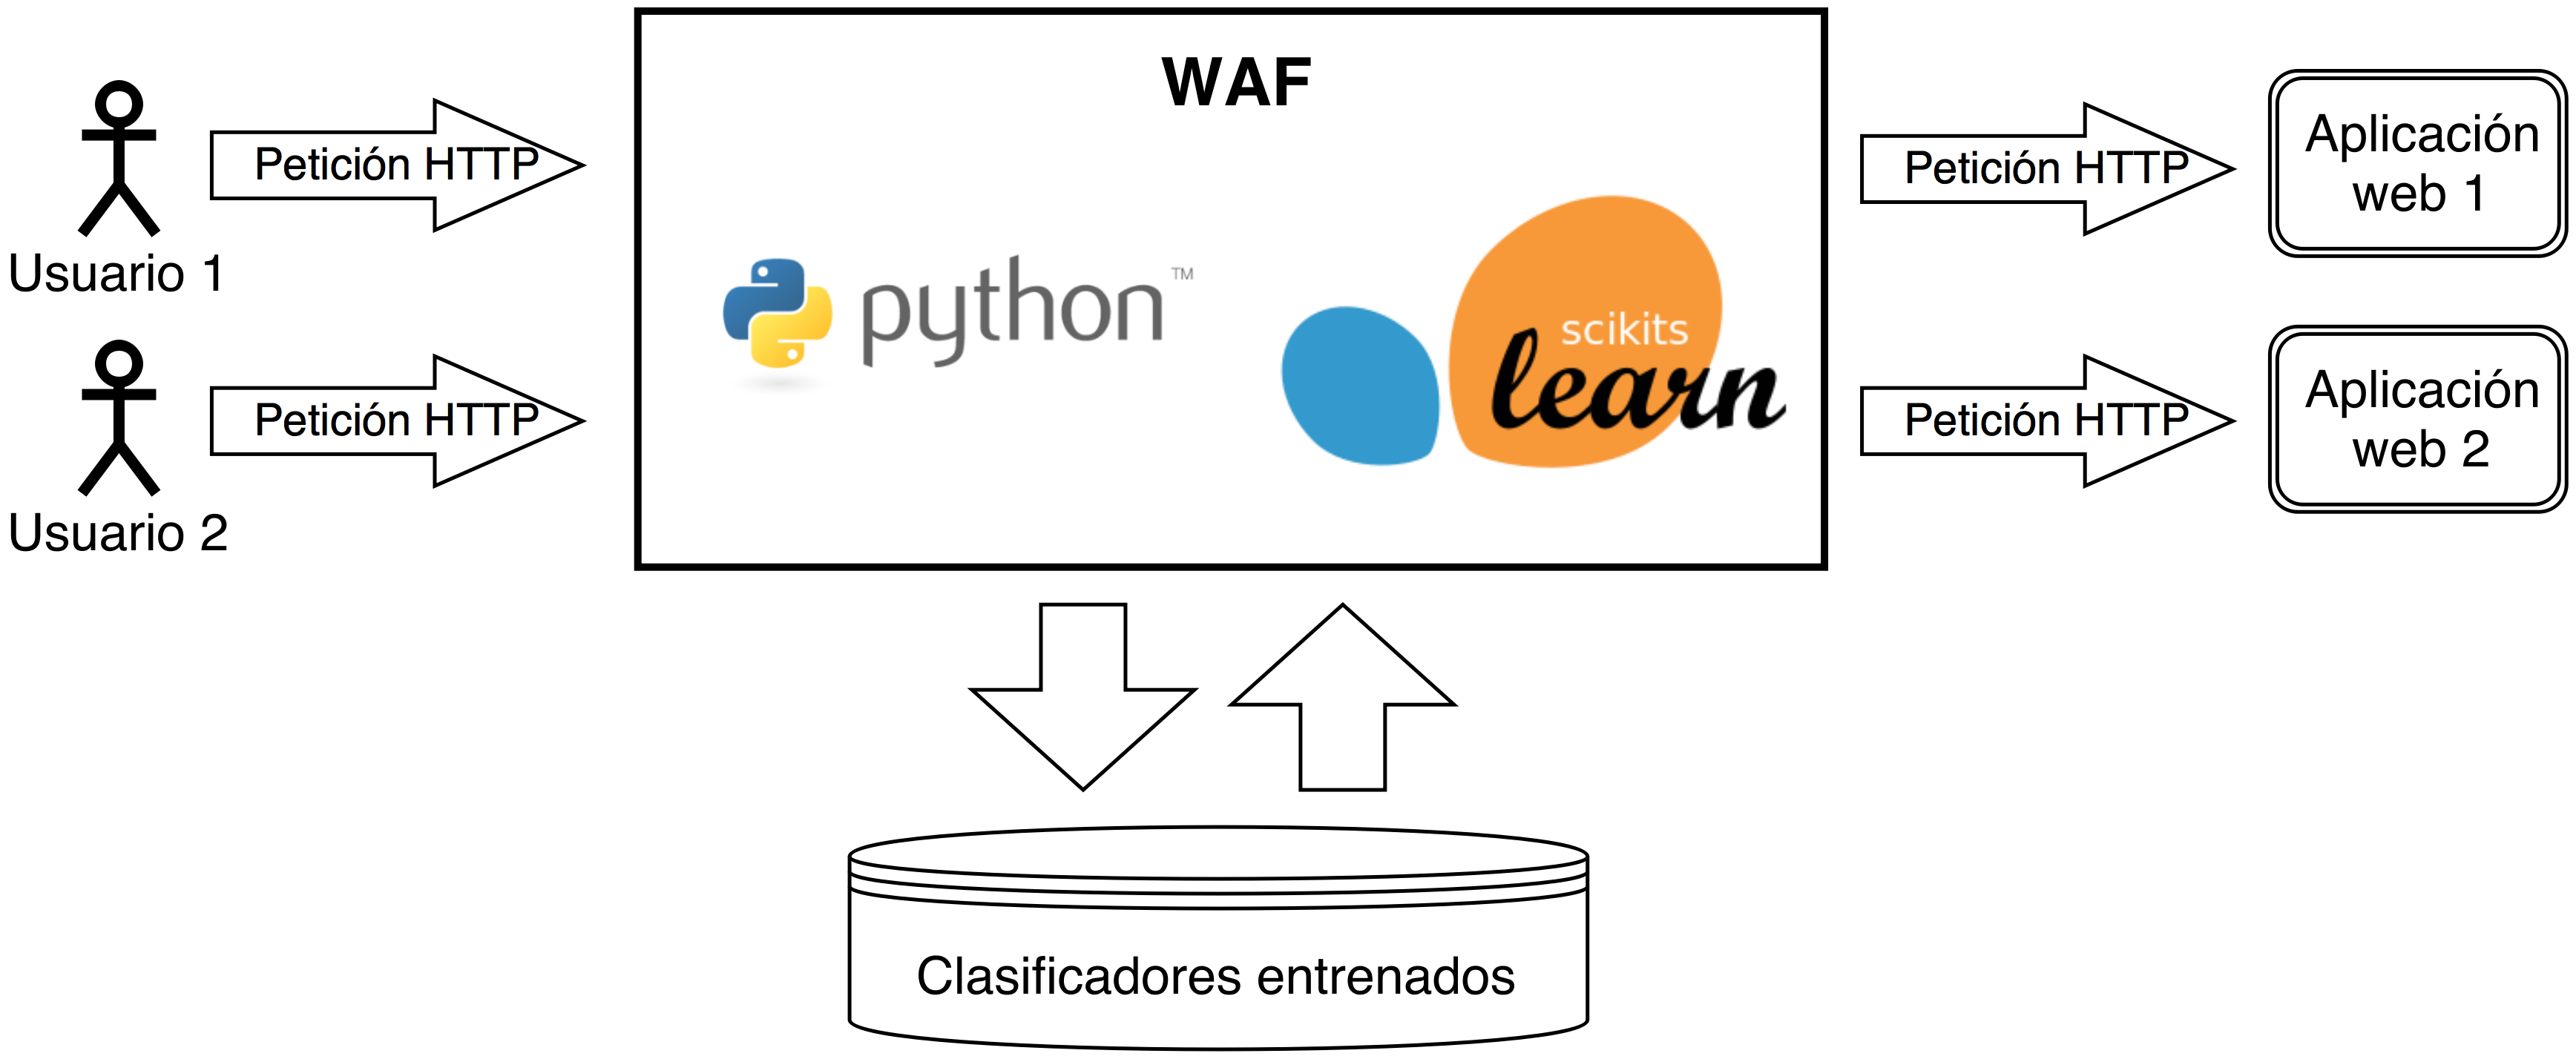
\includegraphics[width=\linewidth]{images/waf-diagram-overview.png}

    \caption{Arquitectura general del funcionamiento de \gls{acr3:name}.}
    \label{fig:waf:waf_diagram_overview}
\end{figure}

\gls{acr3:name} también utiliza la librería \textit{scikit-learn}
\citep{scikit-learn}, que es una librería con herramientas del área de
\gls{acr3:ml} para \textit{Python}. De esta librería se utilizaron varias
herramientas, como por ejemplo, el \textit{BaseEstimator} para implementar
las funciones de extracción de \textit{features}, el \textit{StandardScaler}
para el escalamiento de \textit{features}, el \textit{OneClassSVM} para
el proceso de clasificación y finalmente se emplea el \textit{FeatureUnion}
y el \textit{Pipeline} para coordinar el flujo de datos entre todos estos
componentes.


\section{Fase de entrenamiento}

Esta fase sirve para preparar el \gls{acr3:name} para la detección de
peticiones \gls{acr3:http} anómalas. La \autoref{fig:waf:waf_diagram_training}
muestra la arquitectura de \gls{acr3:name} en esta fase de entrenamiento.
Se utiliza peticiones recolectadas que representan el tráfico normal de
las aplicaciones web, las cuales pasan por tres pasos intermedios durante
esta fase; primeramente se agrupan las peticiones según su método
\gls{acr3:http} y \gls{acr3:url}, luego se realiza el preprocesamiento
de las peticiones y finalmente se entrena los clasificadores dentro de
cada grupo.

\begin{figure}[ht]
    \centering
    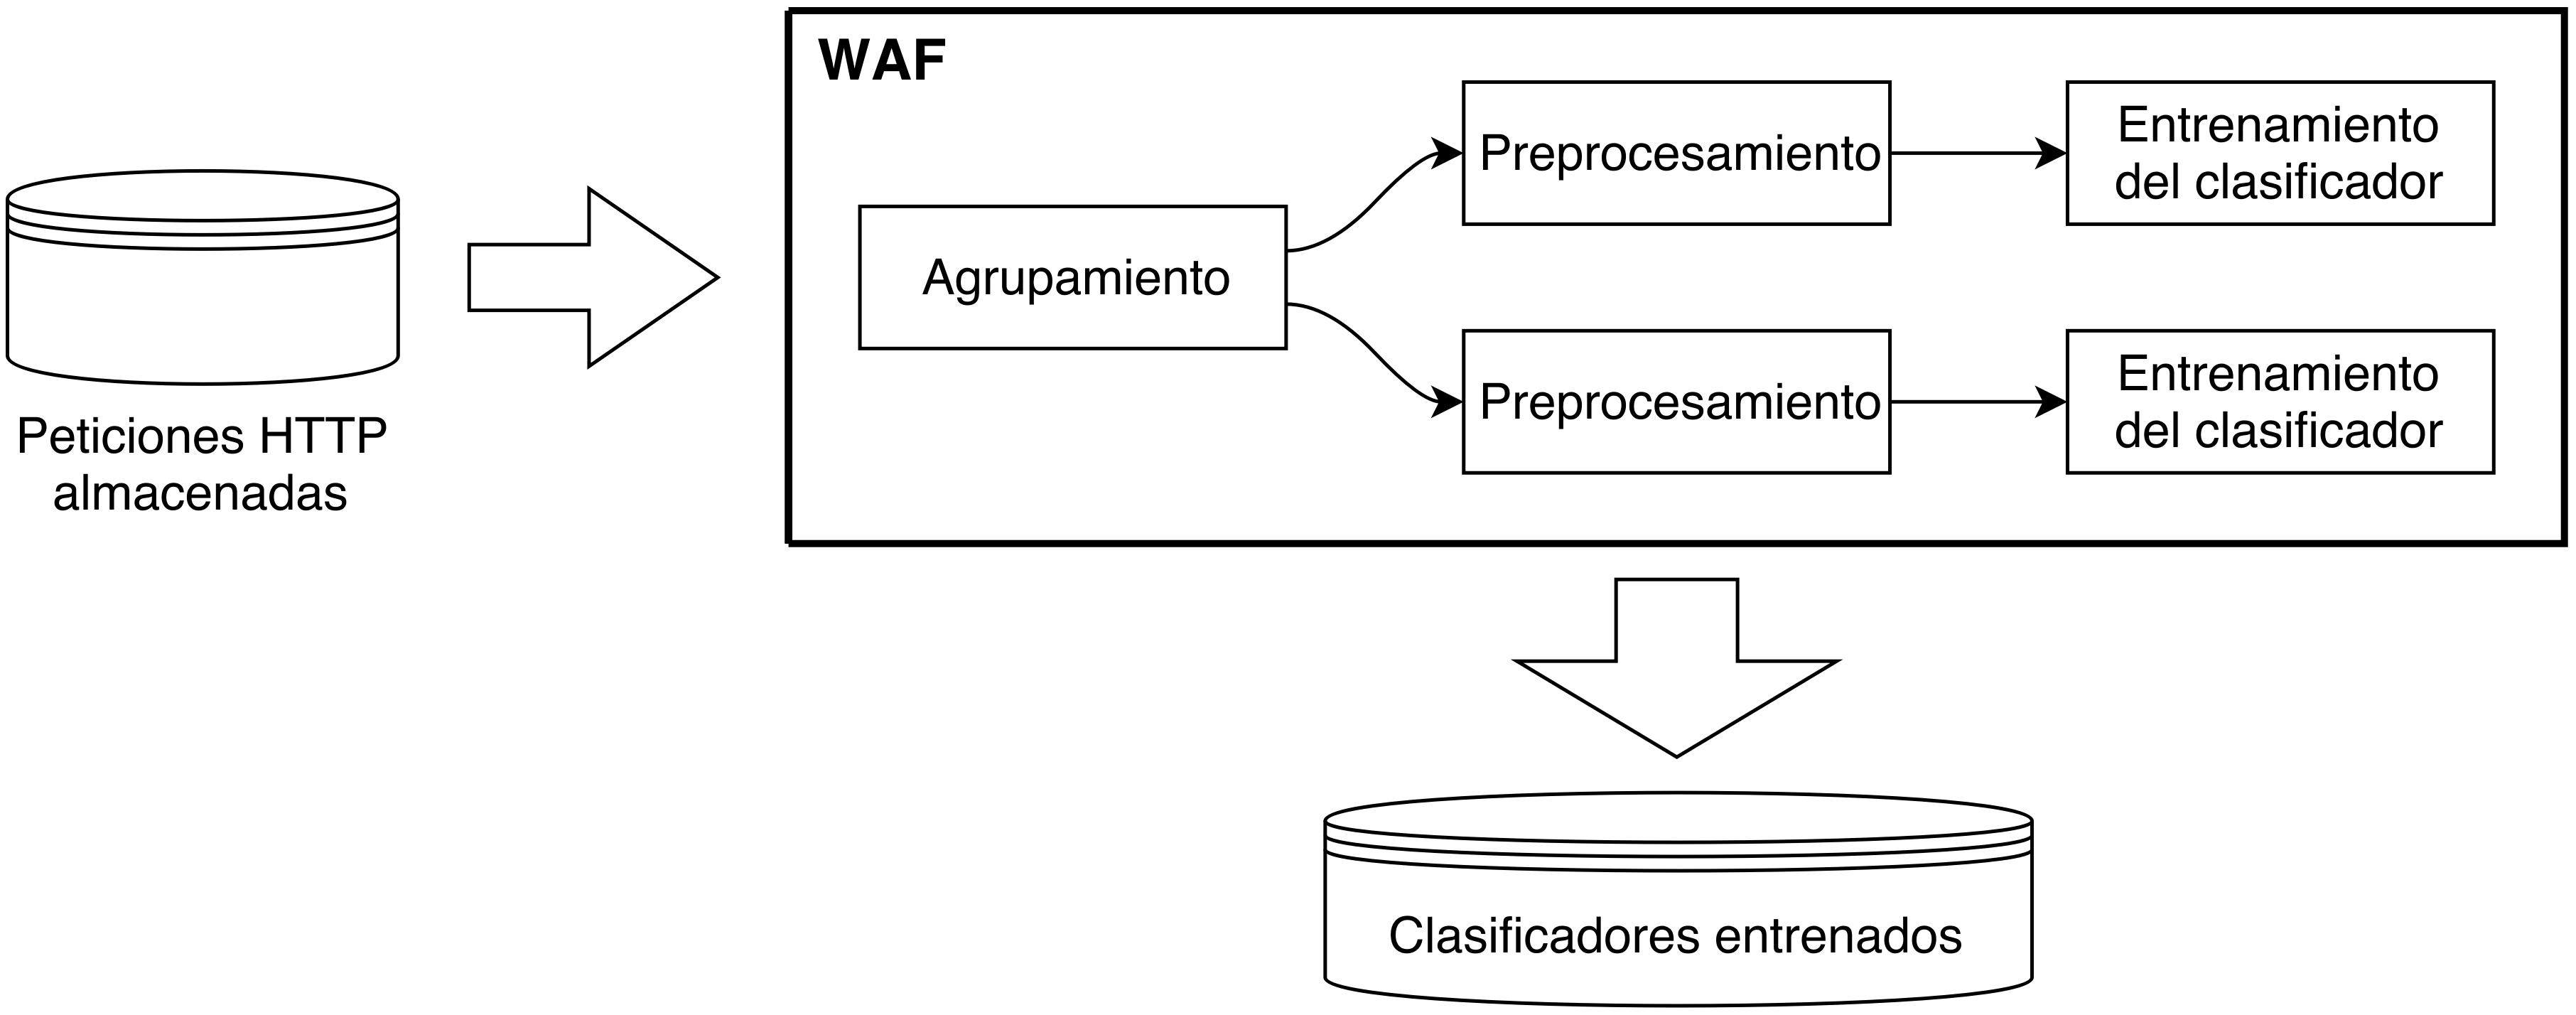
\includegraphics[width=\linewidth]{images/waf-diagram-training.png}

    \caption{Arquitectura de \gls{acr3:name} en la fase de
        entrenamiento.}
    \label{fig:waf:waf_diagram_training}
\end{figure}

Como se puede observar en la figura mencionada, para esta fase se necesitan
peticiones normales (la clase conocida) que representan el tráfico normal
que se espera recibir durante la fase de detección. Se podría usar nuestra
implementación para esta recolección de muestras; para eso se debe proceder
a deshabilitar los procesos de análisis y solamente almacenar las peticiones
que pasen por el detector.


\subsection{Paso de agrupamiento}

Como ya hemos explicado en el \autoref{chap:p3_concepts_features},
agrupamos las peticiones \gls{acr3:http} por método y \gls{acr3:url}
para aprovechar las semejanzas que presentan las peticiones dentro de
un mismo grupo. Partimos de la premisa de que peticiones que van dirigidas
a una misma \gls{acr3:url} y con el mismo método \gls{acr3:http} presentan
más similitudes entre ellas que con peticiones que tienen otro método o
\gls{acr3:url}. Agrupando las peticiones disponibles por método y
\gls{acr3:url} se puede entrenar clasificadores independientes sobre
cada uno de estos grupos. De esta forma se puede obtener modelos de
anomalías más precisos dentro de cada grupo, con el fin de lograr mejores
resultados en la fase de detección.

Utilizando la nomenclatura que hemos introducido en el
\autoref{chap:p3_concepts_features}, podemos denominar \gls{sim3:g} al
conjunto de los grupos de peticiones que se obtienen por este paso de
agrupamiento. Consecuentemente, cada grupo es identificado como \gls{sim3:gi}.


\subsection{Paso de preprocesamiento}

En el paso de preprocesamiento, nuestros procesos de extracción de
\textit{features} son aplicados a las peticiones \gls{acr3:http} para
representarlas con vectores numéricos de \textit{features}.
Este paso se realiza de forma independiente para cada grupo \gls{sim3:gi}.
Debido a eso, en la \autoref{fig:waf:waf_diagram_training} podemos ver
múltiples instancias de preprocesamiento, que corresponden a los distintos
grupos.

Primeramente, como ya hemos explicado en el
\autoref{chap:p3_concepts_features}, \gls{acr3:name} construye las listas
\gls{sim3:qi} y \gls{sim3:bi}, que contienen todos los parámetros que
aparecen en el \textit{query string} y cuerpo de alguna petición dentro
del grupo \gls{sim3:gi}. Las duplicaciones son excluidas, y las listas
son ordenadas de forma alfabética.
Después, nuestra implementación procesa las peticiones de cada grupo
\gls{sim3:gi} para construir los conjuntos de vectores \gls{sim3:fi},
en donde cada petición está representada por un vector de \textit{features}
\gls{sim3:fij}. Así, por cada petición en \gls{sim3:gi}, \gls{acr3:name}
extrae los $m = 10$ \textit{features} de la petición completa, incluyendo
cada una de las seis partes que puede tener dicha petición. Luego se
extraen los valores cuyos parámetros aparezcan en las listas \gls{sim3:qi}
y \gls{sim3:bi}, y se generan $m = 10$ \textit{features} de cada uno de
esos valores.

Los $m = 10$ \textit{features} extraídos analizan distintas características,
que son la distribución de caracteres, la entropía y la cantidad de
caracteres de cada valor. Las funciones utilizadas para la extracción
de estos \textit{features} se encuentran en el directorio
\path{/waf/feature_extraction/} de nuestro repositorio.
Debido a que los \textit{features} ya fueron explicados en detalle en el
\autoref{chap:p3_concepts_features}, a continuación nos limitaremos a una
breve descripción de las tres funciones utilizadas por \gls{acr3:name}
para obtener los \textit{features} para cada valor analizado.

\begin{itemize}
    \item
    \textit{Distribución de caracteres}:
    se calcula la frecuencia relativa de cada carácter, se ordena estas
    frecuencias de forma descendente y se agrupan las mismas en cinco
    intervalos de distintos tamaños.
    Para cada valor analizado, esta función retorna cinco números del
    tipo punto flotante, que corresponden a los cinco intervalos que
    fueron calculados.

    \item
    \textit{Entropía}:
    está función calcula la entropía de un valor según la
    \autoref{eq:fe:entropy}.
    Para cada valor analizado, se retorna un número de tipo punto flotante,
    que corresponde a la entropía calculada.

    \item
    \textit{Cantidad de caracteres}:
    esta función cuenta los caracteres de un valor que pertenecen a
    cuatro categorías definidas, específicamente contando la cantidad
    total de caracteres, la cantidad de dígitos, de letras, y finalmente
    la cantidad de otros caracteres que no sean dígitos ni letras.
    Para cada valor analizado, la función retorna cuatro números de
    tipo punto flotante, que corresponden a las cantidad de las cuatro
    categorías mencionadas.
    Esta función podría retornar números enteros, pero elegimos el tipo
    de dato punto flotante para que se obtenga vectores \gls{sim3:fij}
    homogéneos sin realizar conversiones adicionales posteriormente.
\end{itemize}

Todos los números retornados por estas funciones son concatenados de forma
ordenada para formar el vector \gls{sim3:fij} de cada petición. La dimensión
de estos vectores está definida por la \autoref{eq:fe:number_of_features}.
Cabe resaltar que cada grupo \gls{sim3:gi} puede tener una dimensión
distinta para sus vectores \gls{sim3:fij}, ya que depende de la cantidad
de parámetros de las peticiones del grupo.

Con estos vectores de \textit{features} se construye la matriz \gls{sim3:mi}
de cada grupo, donde los vectores conforman las filas de la matriz.
Luego de obtener la matriz \gls{sim3:mi} del grupo, se procede a escalar
los \textit{features}, que son las columnas de la matriz. Se busca que
cada \textit{feature} tenga promedio cercano a 0 y varianza cercana a 1.

Aclaramos que \gls{acr3:name} puede ser extendido con mucha facilidad
en esta parte de extracción de \textit{features}, agregando o quitando
funciones que analizan los valores.


\subsection{Paso de entrenamiento del clasificador}

Después de realizar la extracción de \textit{features} y el escalamiento
de los mismos, \gls{acr3:name} utiliza las matrices \gls{sim3:mi} obtenidas
para entrenar un clasificador \gls{acr3:ocsvm} para cada grupo \gls{sim3:gi}.
Para el proceso de entrenamiento, el \gls{acr3:ocsvm} recibe la matriz
\gls{sim3:mi} y también los valores para los parámetros \gls{sim3:nui}
y \gls{sim3:gammai} elegidos para ese grupo.
Como ya mencionamos en el \autoref{chap:p3_concepts_ocsvm}, utilizamos
el \textit{kernel} \gls{acr3:rbf} para todos los clasificadores.

Para finalizar esta fase de entrenamiento, \gls{acr3:name} almacena toda
la información necesaria para realizar la detección de anomalías en la
fase de detección. Primeramente se almacenan datos generados por los procesos
de extracción de \textit{features}, que incluye los parámetros extraídos
y su orden dentro de los vectores, luego se persiste los promedios y
desviaciones calculados para el escalamiento de cada \textit{features},
y por último se guarda también el clasificador entrenado.
Nuestra implementación almacenado toda esta información en un archivo
binario en disco, para ser utilizado posteriormente en la fase de detección.

La selección de los valores para los parámetros \gls{sim3:nui} y
\gls{sim3:gammai} presenta un gran desafío. Esto se debe a que durante
la fase de entrenamiento no se cuenta con peticiones anómalas (muestras
positivas) para validar si el clasificador entrenado clasifica correctamente
las anomalías; solamente se puede validarlo contra las peticiones normales.
Esto es un desafío que está presente en los problemas de \gls{acr3:occ},
ya que no se tiene disponible mucho conocimiento sobre las muestras que
no pertenecen a la clase conocida
\citep{khan2009survey}. % from abstract

Una estrategia para encontrar valores adecuados para los dos parámetros
en cuestión puede ser el entrenamiento de un clasificador con solamente
un subconjunto de los datos disponibles, utilizando los datos restantes
para una validación posterior al entrenamiento. Este proceso puede ser
repetido para varios valores distintos de \gls{sim3:nui} y \gls{sim3:gammai},
seleccionando finalmente los valores que resulten en la mejor clasificación
de los datos de entrenamiento.
Utilizamos esta estrategia en las pruebas que realizamos con \gls{acr3:name},
las cuales presentaremos en el siguiente capítulo. Sin embargo, nuestra
implementación no cuenta todavía con un método automático para la selección
de los valores para \gls{sim3:nui} y \gls{sim3:gammai}.


\section{Fase de detección}

En esta fase, \gls{acr3:name} utiliza los procesos de extracción y
los clasificadores entrenados para analizar las peticiones \gls{acr3:http}
entrantes con el fin de determinar si dichas peticiones son normales o
anómalas. Según el resultado de la detección, el \gls{acr3:waf} realiza
distintas acciones configurables para cada caso.

En la \autoref{fig:waf:waf_diagram_detection} se puede observar la
arquitectura de \gls{acr3:name} en esta fase de detección.
Se puede notar cuatro pasos intermedios para esta fase, que son el
enrutamiento de las peticiones a su grupo \gls{sim3:gi} correspondiente,
el preprocesamiento y la clasificación de las mismas, y finalmente las
acciones que son realizadas en respuesta al resultado de la clasificación
de cada petición analizada.

\begin{figure}[ht]
    \centering
    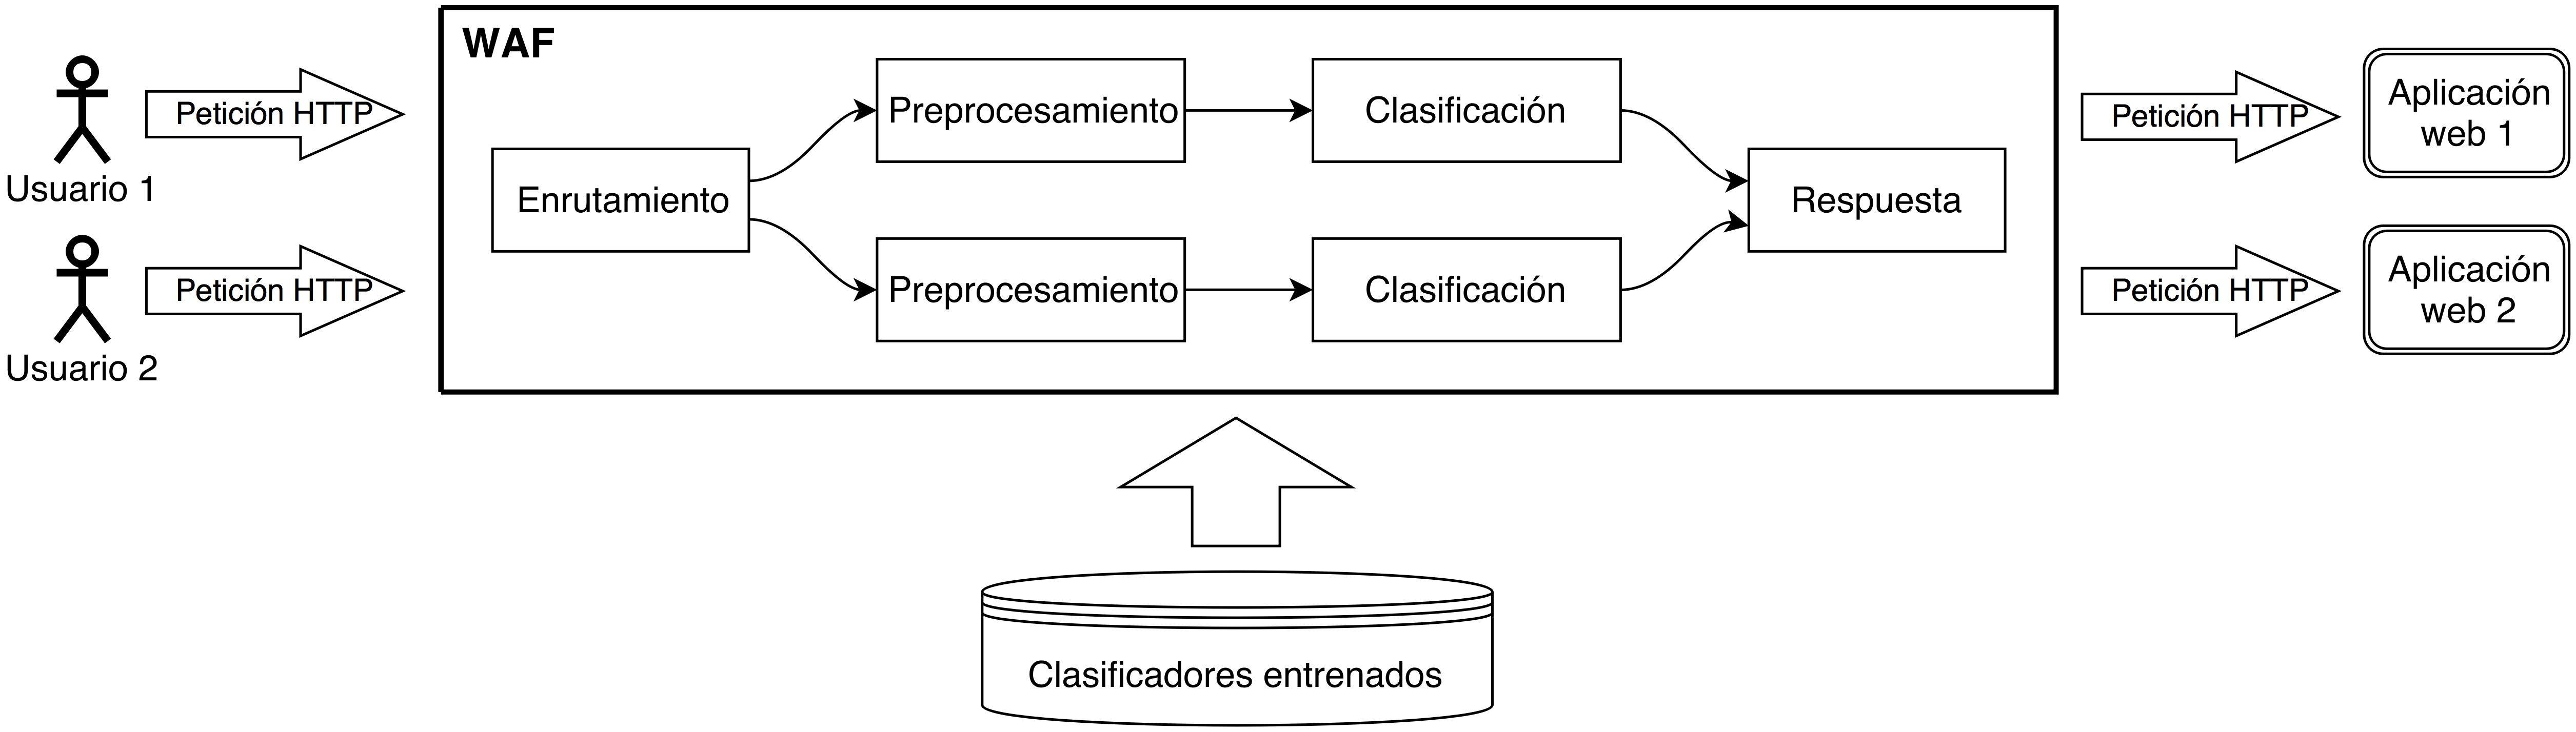
\includegraphics[width=\linewidth]{images/waf-diagram-detection.png}

    \caption{Arquitectura de \gls{acr3:name} en la fase de
        detección.}
    \label{fig:waf:waf_diagram_detection}
\end{figure}


\subsection{Paso de enrutamiento}

Como se puede observar en la \autoref{fig:waf:waf_diagram_detection},
\gls{acr3:name} puede proteger múltiples aplicaciones web y procesar
peticiones de varios usuarios. Los grupos \gls{sim3:gi}, que fueron
formados durante la fase de entrenamiento, pueden ser identificados a
través del método \gls{acr3:http} y la \gls{acr3:url} de sus peticiones.
Para proveer una detección más rápida, \gls{acr3:name} en su proceso de
inicialización ya carga en memoria toda la información almacenada del
entrenamiento, para de esta forma evitar las costosas lecturas de disco
durante el proceso de detección.

De esta forma, este primer paso de enrutamiento determina el grupo
\gls{sim3:gi} correspondiente a cada nueva petición que es recibida
por el \gls{acr3:waf}.
En caso de que no se encuentre el grupo para una petición, \gls{acr3:name}
puede simplemente reenviar dicha petición a su destino por no tener
clasificadores para analizarla, o de lo contrario, puede bloquear dicha
petición por no haber visto peticiones para ese grupo durante el
entrenamiento. Esta configuración queda a cargo de los administradores
responsables por el detector.


\subsection{Paso de preprocesamiento}

Una vez determinado el grupo \gls{sim3:gi} correspondiente a una nueva
petición, \gls{acr3:name} procede a aplicar los procesos de extracción
de \textit{features} a la misma.

Primeramente, se extraen los $m = 10$ \textit{features} de la petición
completa. Luego, utilizando las listas \gls{sim3:qi} y \gls{sim3:bi} del
grupo, los valores de los parámetros de la petición son extraídos y se
generan los $m = 10$ \textit{features} de cada uno.
Atendiendo el orden de los \textit{features}, que fue establecido durante
el entrenamiento, \gls{acr3:name} construye el vector $\vec{x}$ de la
nueva petición. Este nuevo vector tendrá la dimensión correspondiente al
grupo.
Luego se aplica el proceso de escalamiento al vector, usando el promedio
y la desviación estándar calculados para el grupo \gls{sim3:gi}
correspondiente.


\subsection{Paso de clasificación}

En este paso, \gls{acr3:name} emplea el clasificador \gls{acr3:ocsvm}
entrenado del grupo correspondiente para determinar si la nueva petición
será considerada normal o anómala.

El paso de clasificación consiste en aplicar la función de decisión
$g_{i}(\vec{x})$ presentada en la \autoref{eq:ocsvm:decision4} al vector
de \textit{features} $\vec{x}$ que representa a la nueva petición en
cuestión.
Si la clasificación obtiene $g_{i}(\vec{x}) = 1$, entonces la representación
de esta nueva petición en el espacio de dimensiones mayores se encuentra
separada del origen por el hiperplano, indicando que esta petición es
normal (una muestra negativa).
En cambio, si se obtiene $g_{i}(\vec{x}) = -1$, entonces la nueva petición
se encuentra del mismo lado que el origen, indicando que se trata de una
anomalía (una muestra positiva o ataque).


\subsection{Paso de respuesta}

Después de clasificar la nueva petición como normal o anómala, \gls{acr3:name}
procede a realizar las acciones de respuesta que fueron configuradas para
el resultado de clasificación correspondiente.
Si la petición en cuestión es considerada normal, la misma es reenviada
a la aplicación web destino. En cambio, si la petición es considerada
anómala, el resultado de la clasificación y la petición quedan registrados
en un \textit{log}.

Opcionalmente, \gls{acr3:name} puede ser configurado para bloquear las
peticiones anómalas, evitando de esta forma que las mismas lleguen a las
aplicaciones destino. En cambio, si el bloqueo se encuentra deshabilitado,
la petición anómala es reenviada a la aplicación destino, como si fuera
una petición normal.
La configuración del bloqueo de peticiones anómalas queda a cargo de los
administradores responsables, ya que los distintos ambientes de implementación
podrían tener necesidades diferentes. Por ejemplo, ciertos ambientes podrían
preferir bloquear todas las anomalías para evitar posibles ataques. Esto
podría causar que peticiones normales incorrectamente clasificadas no
lleguen a su destino (se producen falsos positivos).
En cambio, otros ambientes podrían optar por solamente lanzar alertas y
no bloquear las anomalías para evitar que peticiones normales erróneamente
clasificadas como anómalas (justamente los falsos positivos mencionados)
no lleguen a su destino y afecten la experiencia de usuarios legítimos.

Además, nuestra implementación puede ser extendida con otras acciones
a realizar en respuesta a la detección de peticiones anómalas. Por ejemplo,
se podría agregar el envío de notificaciones o alarmas en caso de anomalías,
para que los administradores estén enterados al instante y no sea necesario
esperar la inspección de los \textit{logs} para percatarse de distintos
tipos de incidentes de seguridad.


\section{Limitaciones de la implementación}

Nuestra implementación busca ser funcional y sencilla. Se trata de una
prueba de concepto, y por este motivo no nos hemos enfocado en obtener
una aplicación terminada que incluya todas las funcionalidades necesarias
para ser utilizada directamente en ambientes de producción.
A continuación, mencionamos las limitaciones que están presentes en el
\gls{acr3:waf} que implementamos en el marco de este trabajo:

\begin{itemize}
    \item
    \gls{acr3:name} no cuenta con un panel de administración para visualizar
    el estado del mismo o realizar cambios en las configuraciones. Se debe
    realizar el inicio del detector mediante un \textit{script}, utilizando
    parámetros para seleccionar las opciones de configuración.

    \item
    \gls{acr3:name} podría ser utilizado para la recolección de peticiones
    normales para la fase de entrenamiento. Los procesos de detección
    pueden ser deshabilitados indicando la configuración deseada al momento
    de inicialización del \gls{acr3:waf}, pero nuestra implementación
    no cuenta todavía con mecanismos para almacenar las peticiones en
    memoria secundaria.

    \item
    Para el entrenamiento de los clasificadores, \gls{acr3:name} no
    cuenta todavía con un método automático para la selección de los
    valores para los parámetros \gls{sim3:nui} y \gls{sim3:gammai},
    de forma que estos deben ser especificados por los administradores
    del detector.
\end{itemize}

En el siguiente capítulo presentamos las pruebas que realizamos con nuestra
implementación y los resultados que obtuvimos mediante las mismas.
